\documentclass[11pt]{article}
\usepackage{hyperref}
\usepackage[utf8]{inputenc} 
\usepackage[usenames,dvipsnames]{xcolor}
\usepackage{times}
\usepackage[T1]{fontenc}
\usepackage{amssymb,amsmath}
% \usepackage{verbatim}
\usepackage{graphicx}
\usepackage{epstopdf}
\usepackage{url}
\usepackage{listings}
\usepackage{float}
\usepackage[ruled]{algorithm}
\usepackage{algorithmic}

\begin{document}
\title{CSE 592 - Project Report\\
  Hierarchical Co-clustering of Comic Series and their Instances}
\author{
  Chandra Sekhar Mallarapu\\
  Naresh Pratap Singh\\
  Nehal Bandi\\
  \texttt{mcsekhar,mail2naresh,nehal.bandi@gmail.com}}
\date{\today}
\maketitle
\titlepage
\tableofcontents
\listoffigures
\pagebreak

\section{Abstract}
In this Internet age, the number of comics available on the web have exploded. Avid comic readers do not have an easy way to find comics similar to what he/she is interested in. This motivates us to solve the problem of grouping together comics which are similar. We intend to achieve two goals. First, we should be able to tell user which comics in the same series are similar. Second, we should also be able to suggest new interesting comics.
\section{Introduction}
People have been using the medium of comics since a very long time. Comics were traditionally found only in newspapers and print material, for which people had to pay money. But in the present day, a number of people have started their own web based comic series. Another interesting fact is that some of the comics which are printed in newspapers are also available online. Hence, readers are looking more and more to the web for their comic needs. A user who is reading some comic, is naturally interested in finding out other similar comics. We decided to solve this problem by creating groups of similar comics together, as that will aid in future navigation and search.\\
At a first glance, one might think of using image analysis for this. That approach might work with mixed results, if one only wanted similar comics within a series. But, it is neither easy nor promising when attempting to find similarities across various series. Because, images in comics are not standard across series, and are usually very simple and do not represent real world entities faithfully. Another approach is to mine blogs and use search engine results to get information about similarities of comics.\\
Our approach is to use the information in the comic transcripts to find similarities. This is a suitable approach, because in most cases, the transcript contains not just the text of the comics, but also additional details describing the image, scene and setting too. Moreover, one doesn't have to do complex image analysis to understand what the comic is about. And in our opinion, its an easy and better way to understand and analyse the comic. Thus, the transcripts constitute our data samples. We can now do clustering on this data to find out groups of comics similar to each other. We can also use the comic series themselves as samples, and cluster them. Moreover, we decided to go one step ahead and do a hierarchical clustering, as that will allow to create coarse grained clusters too. Since, similarity about comic instances hints at similarity between the comic series they belong to and vice versa, we felt that simultaneously clustering series and instances, also called co-clustering, is a good way to solve the problem described earlier. Thus, the comic series and individual instances from all series constitute our data samples. The features needed will have to be generated from the transcripts of the comics. As we have those transcripts we can use natural language processing techniques to find relevant features and similarity measures. Using that information clusters can be created. The clusters would be useful to find similar comics, as well as browsing comics in general.\\

Eckes et al, \cite{HCC2} have described an algorithm to do hierarchical co-clustering. A modification of this called \emph{HCC} is proposed in Jingxuan Li et al, \cite{HCC1}. We have modified this and used it in our project.

\section{Dataset}
To collect data for our project, we have written a crawler, which downloads the HTML from a web page. We pass it a list of comics series to download. The crawler then searches the web for all the available comic transcripts for that series. It parses them and stores on the disk. This way, we collected transcripts of a few popular comics. The size and distribution of our dataset is as follows:
\begin{itemize}
\item
  About 20528 documents from 9 comic series
\item
  Downloaded following comic series from OhNoRobot\cite{robot}
  \begin{itemize}
  \item
    Calvin And Hobbes - 3696 instances
  \item
    College Roomies From Hell - 2631 instances
  \item
    Diesel Sweeties - 1778 instances
  \item
    Goats - 2266 instances
  \item
    General Protection Fault - 3298 instances
  \item
    Nukees - 889 instances
  \item
    Questionable Content -  1747 instances
  \item
    Sheldon - 3263 instances
  \end{itemize}
\item
  Xkcd - 960 instances\\
  Available from XKCD \cite{xkcd}
\item
  Calvin and Hobbes from GoComics\cite{go}
\end{itemize}

\section{Hierarchical Co-clustering}
We use hierarchial co-clustering which utilizes mutual information between the series and the comics. Document clustering provides additional information for series clustering while series clustering supplements document clustering.
Given two types of data objects $A=\{a_1,a_2,\ldots,a_n\}$ and $B=\{b_1,b_2,\ldots,b_m\}$ and a matrix $X$, such that $x_{ij} \in \mathbb{R}$ represents the relation between $a_i$ and $b_j$. We need to simultaneously cluster objects in $A$ and $B$, and create hierarchies out of those clusters.
Here we describe a modification of the \emph{HCC} algorithm presented in \cite{HCC1}.
We start off with singleton clusters containing a tuple, which is a pair of a single document and a single series. We then combine two nearest clusters in each iteration, until there is only one cluster. Thus, a dendrogram is generated, with the leaves being tuples containing a single document and a single series, and internal nodes containing a cluster of such tuples. At the root, we have all such tuples.
The modified \emph{HCC} algorithm is described below.
\begin{algorithm}[H]
  \caption{HCC Algorithm Description}
  \label{hcc_algo}
  \begin{algorithmic}
    \STATE {Create an empty hierarchy $H$}
    \STATE {$List \leftarrow$ Objects in $A$ $X$ $B$}
    \STATE {$N \leftarrow |A$ $X$ $B|$}
    \FOR{$i=0$ to $N-1$}
    \STATE {$p,q$=PickUpTwoNodes($List$)}
    \STATE {$o$=Merge($p,q$)}
    \STATE {Remove $p,q$ from $List$ and add $o$ to $List$}
    \STATE {Add $List$ to $H$ as next layer}
    \ENDFOR
  \end{algorithmic}
\end{algorithm}
The main step in this algorithm is to find out which two nodes have to be merged, which is what the \emph{PickUpTwoNodes} procedure does. It works as given below.
Given a cluster $C$ with $m$ tuples, the cluster heterogeneity of this cluster $CH(C)$ is defined as:
\begin{displaymath}
  CH(C)=\frac{1}{|C|}\sum_{(a_i,b_j) \in C}(x_{ij}-\mu)^2
\end{displaymath}
where $\mu=\frac{1}{|C|}\sum_{(a_i,b_j) \in C}x_{ij}$.
Another choice for $\mu$ was given in \cite{HCC2} in which they used $\mu=max(x_{ij}), \forall x_{ij} \in X$. We ran our experiment using this measure too.\\
The clusters to be merged are found out by calculating $CH(C_1 \cup C_2)$, for all pairs of clusters $C_1,C_2$ from the current clusters, and picking the pair whose union has minimum $CH(C)$. What we are doing is determining the variance of the newly formed cluster and picking that cluster which will have least variance.\\

\section{HCC for Comic Series and Instances}
We apply the algorithm described above to our problem of creating simultaneously a hierarchical clustering of comic series and instances.
In our case, the sets of objects we have are $S$, the set of comic series and $D$, the set of comic instances from all series. The only detail of the \emph{HCC} algorithm specific to our problem is the relationship matrix $X$.
We used two methods to create this matrix. They are described below.
\subsection{Relationship Matrix using Bag of Words}
We use a \emph{bag of words} approach here. We run a \emph{stemmer} \cite{stemmer} on the transcripts to get the stems of the words present in them. From this list of words(stems), remove \emph{stop words}, i.e., those words which occur in almost all documents and do not convey information that we need about the comic.
\subsubsection{Word and document relationship}
Now, let $W$ represent the set of all words $w_1,w_2,\ldots,w_n$ from all the documents. We create a single corpus out of all the documents in our dataset and calculate the \emph{tfidf} of a word $w_i$ with respect to a document $d_j$, based on this corpus. Lets call that value as $t(w_i)$. This value represents the relationship between $d_j$ and $w_i$ and hence we store it as the value of $x_{ij}$ in the relationship matrix between words and documents.\\
The \emph{tfidf} score of a word $w$ with respect to a document $d$ is calculated based on the corpus $C$ from which this document was taken and is defined as follows:
\begin{align*}
  D(w)&=\textrm{number of documents in the corpus having word } w\\
  freq(w)&=\textrm{frequency of word } w \textrm{ in document } d\\
  tfidf(w)&=freq(w)*\log \Huge(\frac{|D|}{|D(w)|}\Huge)
\end{align*}

We run \emph{HCC} on the words from all the documents and the documents themselves, and use the clusters of words and documents thus generated to calculate the relation between documents and series. But, when we had used this technique in our experiments, we had the words and documents as the leaves of the cluster, instead of tuples. (as mentioned previously in the description of the algorithm)\\
Note that this clustering will take $|W|+|D|-1$ iterations, creating one cluster $C_i$ in iteration $i$, by merging two clusters $C_{i1}$ and $C_{i2}$.

\subsubsection{Document and series relationship}
We need to find out the relationship between documents and series. What connects them is the words in the document and the words in the series. Hence, from the clusters generated above for words and documents, we can determine the relationship between documents and series as follows.
\begin{itemize}
\item
  Initialise all values in the relationship matrix $X$ that stores the relation between documents and series to $0$.
\item
  Let $K=|W|+|D|-1$, where $W$=set of words and $D$=set of documents
\item
  For clusters $C_{i1}$ and $C_{i2}$ that were merged in iteration $i$ of the algorithm that was run previously for co-clustering words and documents,
  \begin{itemize}
  \item
    $K=K-1$
  \item
    For each document $d_i$ in $C_{i1}$
    \begin{itemize}
  \item
    For each series $s_j$ that each documents in $C_{i2}$ belong to, do the following
        $$x_{ij}=x_{ij}+K$$
\item
      Do the same for $C_{i2}$
\end{itemize}
  \end{itemize}
\end{itemize}
What we have done above is utilised the clusters of words and documents created by co-clustering, to obtain values for relationship between series and documents. And since the similarity decreases as we move up along the hierarchy, we keep decreasing the magnitude that we keep adding to the relationship strength between the documents and series present in any word-document cluster.


\subsection{Relationship Matrix using LMs}
In this case, the rows of the relationship matrix $X$ are the documents and the columns are the series $S$. We use \emph{language models} in this method. Language models are a probabilistic way of describing a corpus of text. An \emph{ngram} is a sequence of $n$ words in a text. Viewing all documents from a series $s_i$ as a corpus, we create a \emph{ngram} language model(LM) $nLM_i$ from that corpus, where the $n$ in $nLM_i$ denotes how many \emph{ngrams} were used for creating that model. We do this for all series in our dataset, thus creating as many LMs as the number of series.\\\\
The perplexity of a given text $t$ with respect to a language model $L$ is defined as $\sqrt[N]{\frac{1}{P(t)}}$ where $P(t)$ is the probability of $t$ with respect to the LM $L$ and $N$ is the number of words in $t$. Perplexity is a measure of how likely this text could have come from that LM. A high perplexity means that the LM was surprised by that text.
For each document $d_i$, we calculate the perplexity of the document with respect to the LM $nLM_j$ created using the series $s_j$. Let $p_{ij}$ denote this value.
Since perplexity denotes the inverse of the likelihood of the text with respect to a LM, we decided that $\frac{1}{perplexity}$ is a measure of how related a document is to a series. Thus, we store $\frac{1}{p_{ij}}$ as the value of $x_{ij}$ in the relationship matrix $X$. \\
We used NLTK \cite{nltk} for constructing these language models.

\section{Results and Discussion}
\begin{figure}[H]
  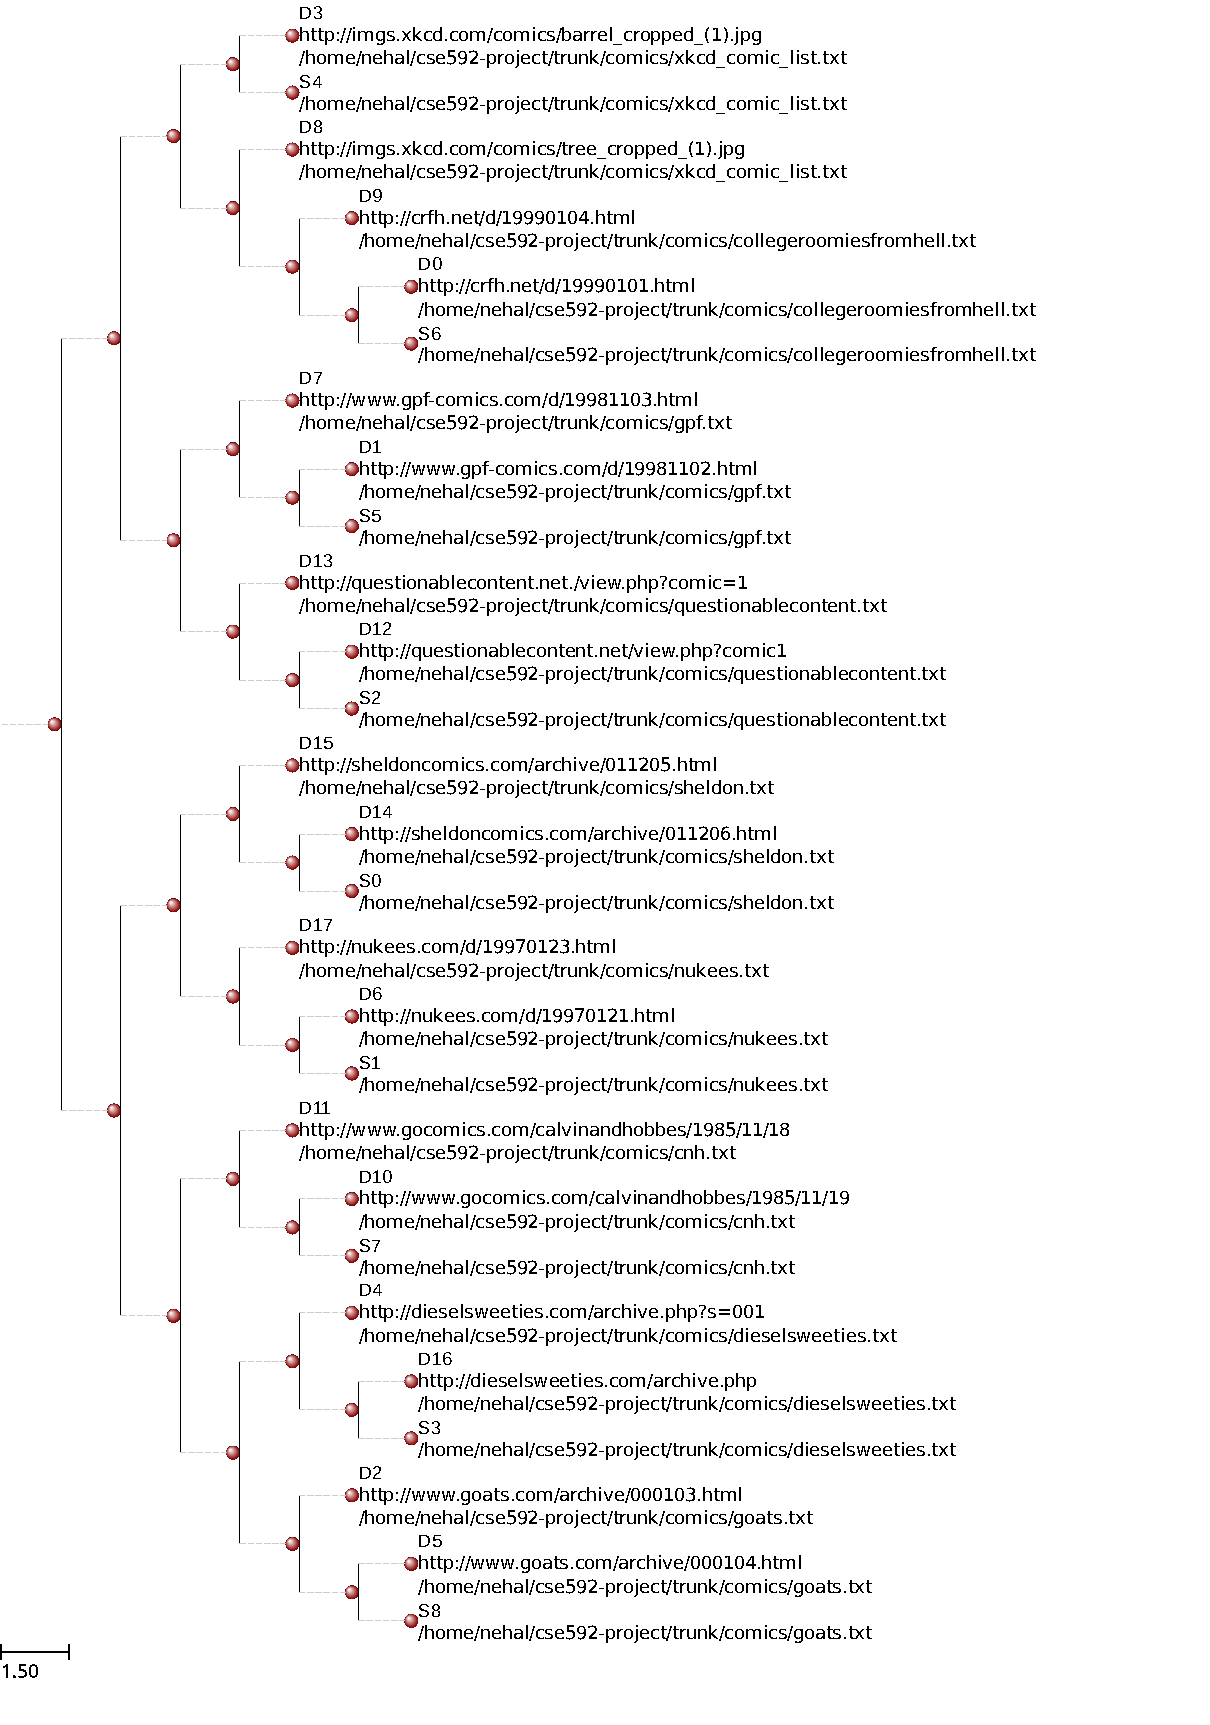
\includegraphics[scale=0.4]{demo1.pdf}
  \caption{Dendrogram of hierarchical co-clustering using Bag of Words}
\end{figure}

 \begin{figure}[H]
   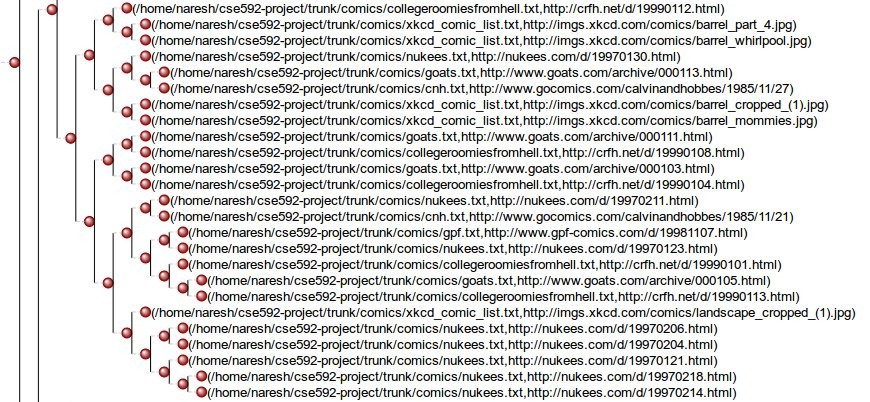
\includegraphics[scale=0.4]{DiffTree}
   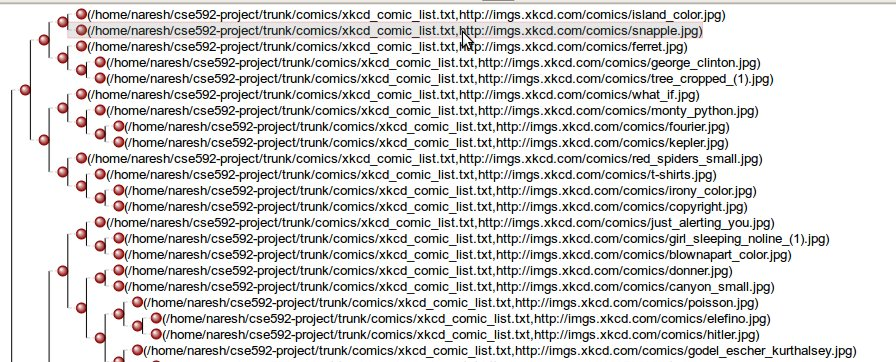
\includegraphics[scale=0.4]{SameTree}
   \caption{Dendrogram of hierarchical co-clustering using 1-gram Language Model}
 \end{figure}
We have shown fragments of two dendrograms. The first one is from our Bag Of Words model which used the co-clustering information from word-docuemnt cluster to create document-series cluster. The results look promising. Our technique clustered most of the comics from same series together. This indicates that comics from the same series use similar writing style, words etc. We also noticed comics from different series were clustered together. For example, instances from series $S6$ - \emph{College Roomies From Hell} were clustered with that series, and then grouped with $S4$ - \emph{XKCD}. This also reflects reality because they are in fact related to college life. We thus see a simultaneous clustering of comic series and instances.\\\\
The second figure shows two fragments of dendrogram generated by our second approach which used language models for each series. The first fragment shows comics from different series getting clustered together. These comics have some similarity. \emph{General Protection Fault} and \emph{XKCD} are related as they have mentions of software and other related information technology terms. Both \emph{College Roomies From Hell} and \emph{XKCD} are related to college life. Second fragment shows the comics of same series (XKCD) grouped together. We ran this algorithm on 900 documents from 9 series.\\\\
In general, our results were satisfactory. We observed similar comics grouping together. We believe the suggestions of similar comics from this cluster would be sensisble and interesting. The success of our approach relies on the usage of similar words in different comic instances. Such similarity is quite strong in the comics from same series. However, it is not very strong across series. Still, the similarity of words is good enough to make interesting suggestions to readers. One additional advantage of hierarchial clustering is it allows users to browse the tree to look for interesting comics. Enabling users to be able to browse comics is a powerful feature which would help them to discover new content on the web.

\section{Future Work}
One area to explore is to use more sophisticated natural language processing techniques to obtain relationship between comic series and instances. Another improvement is that once these clusters are generated, if we wanted to add in new data, the entire process has to be re-done. That turns out to be inefficient, because new data can be added frequently, as new comics are published almost every week. To solve this, we could use the current distribution of series and instances, as prior information and use sequential updating,  to determine into which cluster, new instances and series should be added to.

\begin{thebibliography}{9}
\bibitem{HCC1} Jingxuan Li et al, \emph{HCC: A Hierarchical Co-clustering Algorithm}
\bibitem{HCC2} T. Eckes et al, \emph{An error variance approach to
    two-mode hierarchical clustering}
\bibitem{robot} OhNoRobot \url{http://OhNoRobot.com}
\bibitem{xkcd} XKCD comics \url{http://xkcd.com}
\bibitem{go} GoComics \url{http://gocomics.com/calvinandhobbes}
\bibitem{stemmer} Porter Stemmer \url{http://tartarus.org/martin/PorterStemmer}
\bibitem{nltk} NLTK \url{http://nltk.org}
\end{thebibliography}
\end{document}
